
\section{Desarrollo}


\subsection{Herramientas utilizadas en el proyecto}

Las herramientas utilizadas en este proyecto son QGIS, PostgreSQL y PostGIS.


\subsection{Datos}

Los datos utilizados en esta pŕactica corresponden a las trayectorias de
albatros de Laysan, registradas mediantes dispositivos GPS y GLS
\footnote{Sistema de posicionamiento global y sensor de localización global
respectivamente, por sus siglas en inglés}, de 47 individuos durante los años
2014 a 2018.

Los GPS se programaron para registrar simultáneamente la posición y la velocidad
del albatros cada 20 minutos, lo que permitió grabar de forma contínua durante
12 a 15 días en algunos casos y en otros de 60 a 70 días, durante la etapa
reproductiva \cite{hernandez2019ecologia}.

Para conocer los hábitos migratorios y zonas de distribución en temporada no
reproductiva se instalaron los dispositivos GLS, los cuales fueron recuperados
por lo menos un año después de su instalación.

Los datos crudos se encuentran en formato CSV y contienen los siguientes campos
o atributos:

\begin{table}[h]
\caption{Campos o atributos de los datos crudos de trayectorias de albatros.}
\begin{center}
    \begin{tabular}{ l  m{7cm} }
        \hline
        Atributo & Descripción \\
        \hline
        date & Formato 'yyyy-mm-dd'. Se refiere a la fecha a la cual se registró
        la posición del ave. \\
        \hline
        latitude & Coordenada geográfica de la posición latitudinal del ave. \\
        \hline
        longitude & Coordenada geográfica de la posición longitudinal del ave.
        \\
        \hline
        name & Se refiere al id asociado al individuo de albatros de Laysan.\\
        \hline
    \end{tabular}
\end{center}
\end{table}

\subsection{Identificación del área de anidamiento de la especie}

El albatros de Laysan es una especie que presenta filopatría, esto quiere decir
que generalmente regresa a su colonia natal para reproducirse. En este caso, la
colonia natal de la especie en cuestión es Isla Guadalupe.

Isla Guadalupe es una isla mexicana de origen volcánico, ubicada frente a la
costa de la península de Baja California y tiene una superficie total de
476,971. Está categorizada como Reserva de la Biosfera ha de acuerdo a la
Secretaría de Medio Ambiente y Recursos Naturales y a la Comisión Nacional de
Áreas Naturales Protegidas.

Isla Guadalupe se conforma de una isla principal y tres islotes principales,
Zapato, Morro Prieto y el Toro.

El albatros de Laysan ha establecido sus colonias en la Punta Sur de la Isla
Principal, cuya ubicación se puede observar en la Fig.
(\ref{fig:ubicacionIslaGpe}).

\begin{figure}[h]
    \centering
    \includegraphics[scale=0.60]{figures/Isla Guadalupe.pdf}
    \caption{Ubicación del área de estudio}
    \label{fig:ubicacionIslaGpe}
\end{figure}

\subsection{Creación de base de datos}

Con el fin de visualizar los datos, se cargaron a QGIS como puntos. Se utilizó
la herramienta de clasificación para asignar un color de puntos a cada una de
los individuos monitoreados, como se puede observar en la Fig.
(\ref{fig:trayectorias}).

\begin{figure}[h]
    \centering
    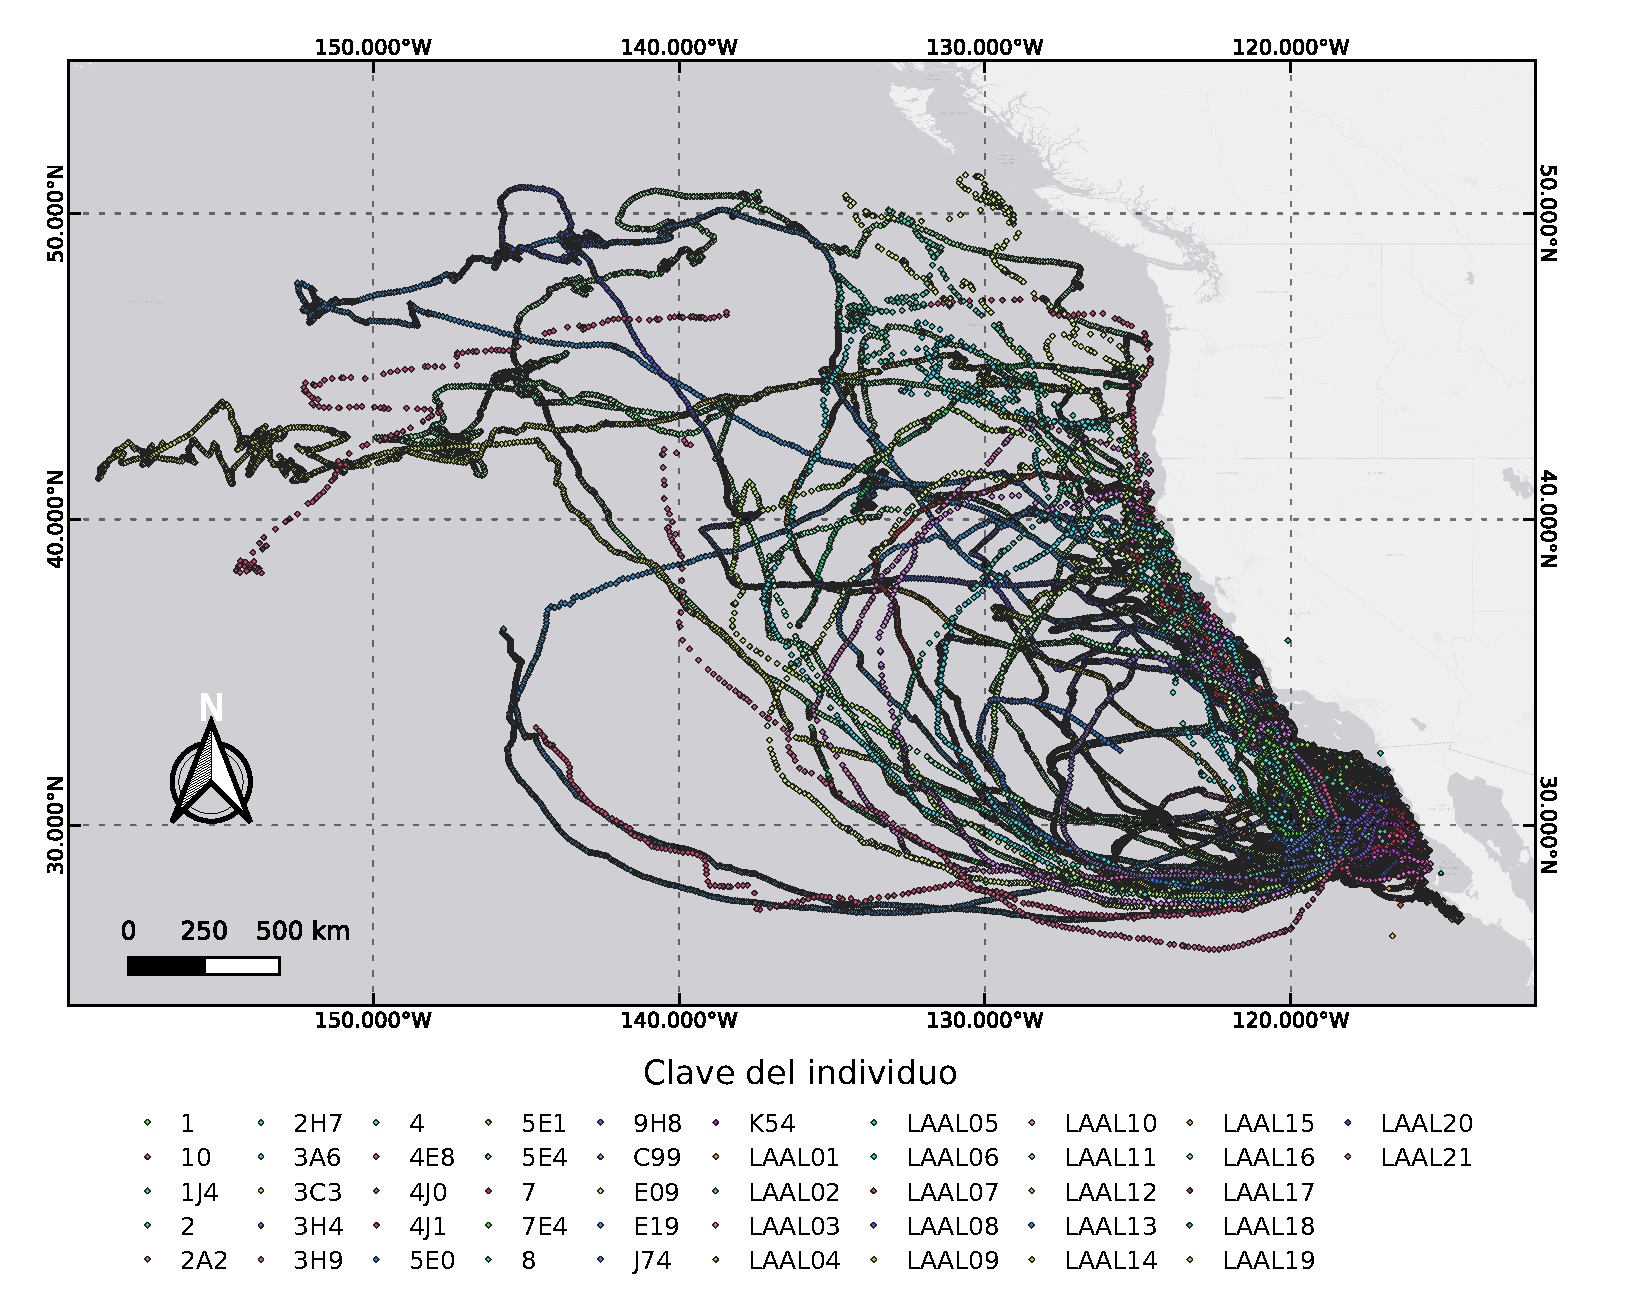
\includegraphics[scale=0.60]{figures/RawData.png}
    \caption{Datos crudos de las trayectorias de albatros}
    \label{fig:trayectorias}
\end{figure}

Como ya mencionamos, QGIS es una herramienta que además de ayudarnos a
visualizar los datos, también nos permite una conexión a una base de datos de
PostgreSQL. En este caso, queremos que todos nuestros datos estén
cargados a una base de datos, por lo que utilizamos en \textit{database
manager}.

Cargamos las siguientes dos tablas a la base de datos:

\begin{itemize}
    \item Tabla de trayectorias de albatros cuya geometría es de tipo punto.
    \item Tabla de poligonos con países del continente americano.
\end{itemize}

En el menú de herramientas:
\texttt{Database} $\rightarrow$ \texttt{DB manager} $\rightarrow$ \texttt{Import
Layer}.

Ahí seleccionamos PostGIS y seleccionamos la base de datos que creamos en
PostgreSQL. Debemos asegurarnos de enviar la capa sobre la que estamos
trabajando y la base de datos en PostgreSQL a la que lo vamos a mandar. Algunos
atributos importantes que debemos seleccionar son el \texttt{id} y
\texttt{geometry column}, ya que estos son los que definirán los atributos
característicos de una base de datos geoespacial.

Otra forma de crear las tablas de la base de datos que estamos trabajando es a
partir de una ejecución de \texttt{SQL command}, en cuyo casó sería como el
código mostado en el anexo.

La ventaja de tener los datos cargados a PostgreSQL es que nos crea un atributo
de tipo \texttt{geometry}. Con este tipo de dato podemos utilizar las funciones
de PostGIS para realizar cálculos u operaciones espaciales, además de realizar
consultas a los datos de manera más facil.

El primer \textit{query} que realizamos fue para agregar una columna con la
temporada de reproducción del individuo, esto con el fin de observar si el rango
de desplazamiento del individuo cambia dependiendo de la etapa reproductiva.

En QGIS:

\texttt{DB manager} $\rightarrow$ \texttt{Database} $\rightarrow$ \texttt{SQL
view} 

\lstinputlisting[language=SQL,   
framesep=10pt, framextopmargin=10pt] {../src/albatross_season.sql}

Al ejecutar este query, obtendremos una vista de los datos con una columna
extra, la cual utilizaremos para visualizar los datos por temporada, además de
que también los podremos cargar como capa a QGIS como se muesta en las Figs.
(\ref{fig:incubacion}, \ref{fig:empollamiento}, \ref{fig:crianza}, y
\ref{fig:NoReproduccion}
).

\begin{figure}[h]
    \centering
    \includegraphics[scale=0.6]{figures/seasonsIncubacion.png}
    \caption{Trayectorias de albatros de Layssan durante la temporada de
    incubación. En esta temporada, los padres alternan entre el ayuno mientras
    incuban el huevo y se alimentan en el mar.}
    \label{fig:incubacion}
\end{figure}


\begin{figure}[h]
    \centering
    \includegraphics[scale=0.60]{figures/seasonsEmpollamiento.png}
    \caption{Trayectorias de albatros de Layssan durante la temporada de
    empollamiento. En esta temporada, las parejas reproductoras alternan entre
    el ayuno en el nido y la alimentación en el mar, donde también aprovisionan
    para el pollito.}
    \label{fig:empollamiento}
\end{figure}

\begin{figure}[h]
    \centering
    \includegraphics[scale=0.60]{figures/seasonsCrianza.png}
    \caption{Trayectorias de albatros de Layssan durante la temporada de
    crianza. Las parejas reproductoras se alimentan de forma independiente en el
    mar y regresan al nido periódicamente para aprovisionar al polluelo.}
    \label{fig:crianza}
\end{figure}

\begin{figure}[h]
    \centering
    \includegraphics[scale=0.60]{figures/seasonsNoReproduccion.png}
    \caption{Trayectorias de albatros de Layssan durante la temporada de no
    reproducción.}
    \label{fig:NoReproduccion}
\end{figure}

\subsection{Uso de las heramientas de procesamiento geo-espacial}

Para hacer uso de las herramientas de procesamiento geo-espacial que nos ofrece,
decidimos calcular la envolvente convexa para todas las trayectorias de los
albatros. Esto con el fin de determinar el área máxima que volaron los albatros
aproximadamente durante todas sus temporadas. Ver Fig. (\ref{fig:fullConvexHull}).

La función utilizada para generar la envolvente convexa es
\texttt{ST\_Convexhull} y en conjunto con \texttt{ST\_Collect} y
\texttt{ST\_astext} se usa de la siguiente manera:

\lstinputlisting[language=SQL,   
framesep=10pt, framextopmargin=10pt] {../src/full_convex_hull_albatross.sql}

\begin{figure}[h]
    \centering
    \includegraphics[scale=0.60]{figures/fullConvexHull.png}
    \caption{Envolvente convexa para las trayectorias completas de los albatros.}
    \label{fig:fullConvexHull}
\end{figure}

Para precisar un poco más el área de desplazamiento, obtuvimos la diferencia del
polígono obtenido anteriormente con el polígono del continente. Esto lo hicimos
ya que al ser aves marinas estas evitan en medida de lo posible el continente.

La función de PostGIS utilizada para generar este resultado es
\texttt{ST\_Difference} y la usamos de la siguiente manera:

\lstinputlisting[language=SQL,   
framesep=10pt, framextopmargin=10pt] {../src/diferencia_query.sql}

El resultado se muestra en la Fig. (\ref{fig:differenceFullConvexHull}).

\begin{figure}[h]
    \centering
    \includegraphics[scale=0.60]{figures/differenceFullConvexHull.png}
    \caption{Envolvente convexa sin área de continente para las trayectorias
    completas de los albatros.}
    \label{fig:differenceFullConvexHull}
\end{figure}


Un análisis semejante se hizo para cada una de las temporadas, esto con el fin
de determinar su área de desplazamiento durante cadá etapa de reproducción Figs.
(\ref{fig:convexHullIncubacion}, \ref{fig:convexHullEmpollamiento} y
\ref{fig:convexHullCrianza}).

\begin{figure}[h]
    \centering
    \includegraphics[scale=0.60]{figures/convexHullIncubacion.png}
    \caption{Envolvente convexa sin área de continente para las trayectorias
    de los albatros durante la temporada de incubación.}
    \label{fig:convexHullIncubacion}
\end{figure}

\begin{figure}[h]
    \centering
    \includegraphics[scale=0.60]{figures/convexHullEmpollamiento.png}
    \caption{Envolvente convexa sin área de continente para las trayectorias
    de los albatros durante la temporada de empollamiento.}
    \label{fig:convexHullEmpollamiento}
\end{figure}

\begin{figure}[h]
    \centering
    \includegraphics[scale=0.60]{figures/convexHullCrianza.png}
    \caption{Envolvente convexa sin área de continente para las trayectorias
    de los albatros durante la temporada de crianza.}
    \label{fig:convexHullCrianza}
\end{figure}

